\subsection{Ablations}
\label{sec:ablations}

\begin{table*}[t]
\centering\small
\caption{Ablations on fold A. All variants share tokens, decoder, optimiser and schedule. Along-ray and lateral are the two components of the endpoint error (mm). Training time is on one Apple M5; inference time is per frame excluding the frozen encoder and including metric computation. The variant without likelihood terms cannot use precision fusion and averages the heads; the geometric-only variant has no direct head.}
\label{tab:ablation}
\footnotesize\setlength{\tabcolsep}{4pt}
\begin{tabular}{@{}lrrrrrrrrrr@{}}
\toprule
Variant & ADE & acc@10 & acc@50 & acc@100 & SD & along ray & lateral & Params (M) & Train (h) & Infer.\ (ms) \\
\midrule
Direct regression, single view & 49.58 & 0.213 & 0.742 & 0.898 & 35.75 & 23.43 & 39.77 & 14.9 & 1.1 & 9.1 \\
Direct, stereo, no ray encoding & 47.47 & 0.205 & 0.754 & 0.908 & 34.78 & 21.84 & 38.47 & 14.9 & 1.7 & 12.0 \\
Direct, stereo + rays (B3) & 46.15 & 0.227 & 0.756 & 0.912 & 33.22 & 22.29 & 36.65 & 15.1 & 2.2 & 12.4 \\
\quad same, seed 1 & 45.73 & 0.222 & 0.776 & 0.918 & 33.40 & 21.55 & 36.66 & 15.1 & 1.8 & 12.3 \\
FIF, geometric head only & 55.11 & 0.097 & 0.689 & 0.896 & 44.11 & 25.71 & 44.31 & 15.1 & 1.9 & 21.8 \\
FIF, mean fusion & 48.38 & 0.173 & 0.747 & 0.911 & 32.48 & 23.28 & 38.53 & 15.1 & 2.4 & 21.4 \\
FIF, no likelihood terms (mean fusion) & 46.48 & 0.169 & 0.757 & 0.921 & 32.41 & 22.44 & 36.79 & 15.1 & 2.3 & 21.3 \\
FIF, no auxiliary losses & 45.71 & 0.207 & 0.774 & 0.920 & 34.09 & 22.29 & 36.27 & 15.1 & 2.2 & 21.3 \\
FIF, single view & 45.19 & 0.219 & 0.783 & 0.918 & 33.32 & 21.46 & 35.86 & 15.1 & 1.3 & 18.2 \\
FIF, learned gate fusion & 44.49 & 0.211 & 0.782 & 0.924 & 32.32 & 21.89 & 34.93 & 15.4 & 2.3 & 21.2 \\
FIF, precision fusion (full) & 44.43 & 0.211 & 0.768 & 0.921 & 31.19 & 21.76 & 35.08 & 15.1 & 2.4 & 21.9 \\
\quad same, seed 1 & 43.82 & 0.221 & 0.787 & 0.927 & 31.87 & 21.46 & 34.50 & 15.1 & 2.4 & 22.4 \\
\bottomrule
\end{tabular}

\end{table*}

\begin{figure}[t]
\centering
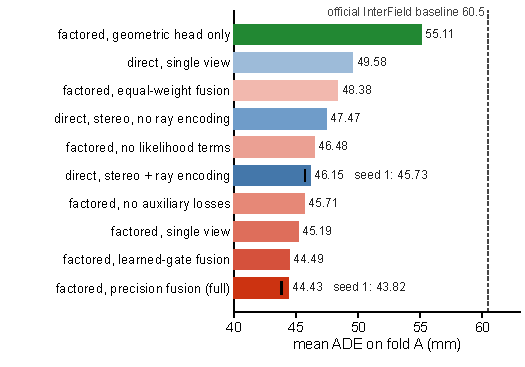
\includegraphics[width=\columnwidth]{../figures/fig8_ablation_ladder.pdf}
\caption{Fold-A held-out ADE of every trained variant, sorted. Vertical ticks mark the second seed of the two main rows; the dashed line is the organisers' InterField result on the same split.}
\label{fig:ladder}
\end{figure}

\Cref{tab:ablation} and \cref{fig:ladder} remove one component at a time. Three findings stand out and each corrects a claim one might otherwise be tempted to make.

\paragraph{The geometric head is not competitive alone}
The geometric head by itself reaches 55.11\,mm, worse than the single-view direct regressor, with acc@10 collapsing to 0.097: forced to reconstruct every field from predicted joints and a predicted pose, it inherits the errors of both arguments and adds none of the direct head's pixel-level precision. The hybrid at 44.43\,mm is better than either of its components, which is genuine complementarity, but the geometric route should not be pitched as a standalone estimator.

\paragraph{Adaptive weighting matters; the precision formulation specifically does not}
Averaging the two heads with equal weights gives 48.38\,mm, worse than the direct regressor alone: mixing a strong estimator with a weak one at a fixed ratio destroys value. Any adaptive weighting recovers it, and the two adaptive rules we trained are indistinguishable: precision fusion reaches 44.43\,mm and a learned sigmoid gate 44.49\,mm, a difference of 0.06\,mm, with the gate slightly better on acc@50 and acc@100. The ablation therefore supports the claim that per-joint adaptive weighting is necessary, and does not support the claim that likelihood-derived weights are better than learned ones. What the precision formulation offers over the gate is a calibrated per-joint uncertainty as a by-product, examined in \cref{sec:inside}.

\paragraph{The likelihood terms pay only through the fusion they enable}
Removing the two Gaussian negative log-likelihood terms from the objective forces equal-weight fusion and gives 46.48\,mm. Comparing this variant with the equal-weight variant that keeps the likelihood terms (48.38\,mm) isolates the effect of the terms at a fixed fusion rule: they make the model 1.9\,mm \emph{worse}. The likelihood objective is not a better regression loss than the plain endpoint error; its value lies entirely in producing the precisions that adaptive fusion consumes, and only the pair of likelihood terms and precision fusion reaches 44.43\,mm.

\paragraph{Auxiliary losses and views}
Removing the joint, object and visibility losses costs 1.3\,mm (45.71 against 44.43): supervising the arguments of $G$ helps even though only the field is evaluated. The single-view factored model at 45.19\,mm loses 0.8\,mm to its stereo counterpart, against 3.4\,mm for the direct regressors, so the factored representation recovers most of what the second camera provides. The factored model costs 1.8 times the inference time of the direct model (21.9 against 12.4\,ms per frame excluding the frozen encoder), almost entirely in the soft nearest-vertex operator over 1,024 vertices, and adds no parameters beyond the two small heads (15.1\,M trainable in both cases).

\subsection{Inside the factored model}
\label{sec:inside}

\begin{table*}[t]
\centering\small
\caption{What each part of the factored model contributes, mean ADE in mm on the held-out subjects. \emph{Standalone direct} is the direct regressor trained without a geometric head; \emph{direct head} and \emph{geometric head} are the two heads of the factored model evaluated separately; \emph{Geo., GT object} and \emph{Geo., GT joints} evaluate the geometric head with the predicted object pose or the predicted joints replaced by their ground truth; \emph{fused} is the model's output. The last two columns give the median fusion weight on the geometric head and the fraction of joints at which its predicted log-scale sits at the clamp of 5 (a standard deviation of 148\,mm).}
\label{tab:oracle}
\footnotesize\setlength{\tabcolsep}{3.5pt}
\begin{tabular}{@{}lrrrrrrrr@{}}
\toprule
Model & Direct alone & Direct head & Geo.\ head & Geo., GT object & Geo., GT joints & Fused & med.\ $w^{\rm geo}$ & $s^{\rm geo}$ saturated \\
\midrule
FIF, fold A, seed 0 & 46.15 & 44.55 & 55.11 & 46.46 & 51.35 & \textbf{44.43} & 0.03 & 100\% \\
FIF, fold A, seed 1 & 45.73 & 43.98 & 56.72 & 45.97 & 50.14 & \textbf{43.82} & 0.03 & 100\% \\
FIF single view, fold A & 49.58 & 45.06 & 58.00 & 44.67 & 48.79 & \textbf{45.19} & 0.04 & 100\% \\
FIF, fold B & 35.68 & 34.29 & 41.47 & 35.08 & 43.11 & \textbf{34.08} & 0.13 & 4\% \\
FIF gate fusion, fold A & 46.15 & 44.86 & 52.58 & 42.69 & 48.27 & \textbf{44.49} & 0.32 & 0\% \\
FIF, SHOW3D+HOT3D, fold A & 46.20 & 45.99 & 62.38 & 47.63 & 54.78 & \textbf{46.16} & 0.03 & 100\% \\
\bottomrule
\end{tabular}

\end{table*}

\begin{figure}[t]
\centering
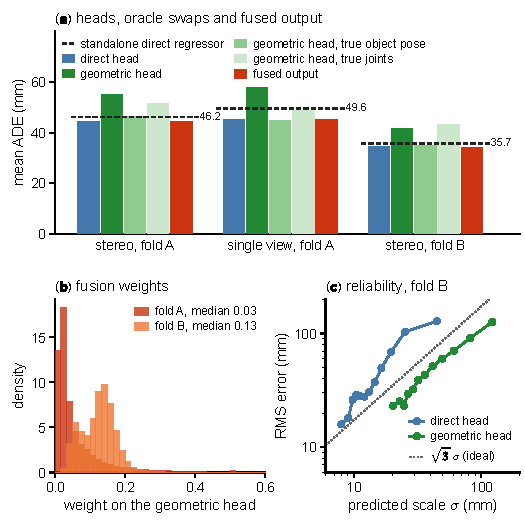
\includegraphics[width=\columnwidth]{../figures/fig7_decomposition.pdf}
\caption{What each part of the factored model contributes. (a) Error decomposition of \cref{tab:oracle} for three factored models; the dashed line is the standalone direct regressor trained without a geometric head. The fused output tracks the direct head to within 0.2\,mm, and the direct head is below the standalone baseline by 1.4 to 4.5\,mm. (b) Distribution of the fusion weight on the geometric head: on fold A the geometric log-scale saturated at its clamp and the weights collapse near zero; on fold B both scales trained normally. (c) Reliability of both heads on fold B, where the geometric scale saturated at only 4\% of joints: binned predicted scale against the root-mean-square error of the residual, with the $\sqrt{3}\sigma$ line an isotropic Gaussian would follow.}
\label{fig:decomp}
\end{figure}

Because the factored model exposes its intermediate quantities, we can ask where its improvement actually comes from. \Cref{tab:oracle} and \cref{fig:decomp} report the two heads separately, the geometric head with each argument replaced by its ground truth, and the behaviour of the learned precisions. The picture that emerges differs from the mechanism one would assume from \cref{eq:fusion}, and we state it plainly.

\paragraph{The improvement is carried by the direct head}
On fold A the direct head \emph{inside} the factored model reaches 44.55\,mm on its own, 1.6\,mm better than the standalone direct regressor trained without a geometric head (46.15\,mm); the same holds for the second seed (43.98 against 45.73), for the single-view model (45.06 against 49.58, a difference of 4.5\,mm) and for fold B (34.29 against 35.68). The fused output improves on the direct head by only 0.12, 0.16, $-0.13$ and 0.21\,mm respectively. In other words, the geometric head and the auxiliary losses act as a structured multi-task signal that shapes the shared decoder, and the direct head reaps the benefit; the combination at inference time contributes about a tenth of a millimetre. This reframes the method: what is being tested is the value of \emph{geometric supervision} for a direct regressor, and that value is 1.4 to 4.5\,mm depending on the setting.

\paragraph{The object pose is the bottleneck of the geometric route}
The geometric head alone gives 55.11\,mm on fold A. Replacing its predicted object pose by the ground truth lowers this to 46.46\,mm, whereas replacing the predicted joints by the ground truth lowers it only to 51.35\,mm: the object pose accounts for about 8.7\,mm of the geometric head's error and the joints for about 3.8\,mm. Even with a perfect object pose, the geometric route (46.46\,mm) does not beat the direct head (44.55\,mm), because the predicted joints are themselves off by roughly the amount that SHOW3D's own hand annotations are~\cite{rim2026show3d}. The object pose dominates on fold B and in the single-view model as well (41.47, 35.08, 43.11 and 58.00, 44.67, 48.79), with the difference that on fold B replacing the predicted joints by their ground truth raises the error slightly rather than lowering it. A better object-pose branch is where the geometric route has room to improve; a better joint branch has little to offer.

\paragraph{The geometric scale saturated on fold A}
In the three SHOW3D-only fold-A precision-fusion runs the geometric log-scale $s^{\text{geo}}$ sits at its upper clamp of 5 for 100\% of joints, a constant predicted standard deviation of 148\,mm. The optimiser found it cheaper to declare the geometric head maximally uncertain everywhere than to calibrate it, which drives the fusion weight on the geometric head to a median of 0.03 and a maximum of 0.50 and explains why the fused output is the direct head to within a fraction of a millimetre. On fold B the same architecture trained normally: the geometric scale has a median of 33.8\,mm, correlates with the head's error (Spearman 0.66) with a log-log reliability slope of 1.00 (\cref{fig:decomp}c), and the median fusion weight is 0.13. The learned-gate variant, whose scales do not enter the fusion, also trained normally (median geometric scale 22.6\,mm, Spearman 0.69). The saturation is thus a training pathology of the precision-fusion objective on this fold, not a property of the geometric head, and the result of \cref{tab:main} was obtained \emph{despite} it, which is a further reason to attribute the gain to the representation rather than to the fusion. We did not intervene on the clamp once the pathology was found, because doing so on the held-out subjects would have compromised the protocol; a wider clamp or a scale-specific learning rate are the obvious remedies.

\begin{table*}[t]
\centering\small
\caption{Calibration of the learned scales. $\rho$ is the Spearman correlation between the predicted standard deviation and the absolute error of the corresponding head (const.: the scale is constant); \emph{remove $k$\%} is the ADE of the joints that remain after discarding the $k$\% with the largest predicted fused scale (in parentheses: after discarding by true error, the oracle); AUSE is the area between the two sparsification curves over the first half of the joints.}
\label{tab:uncertainty}
\begin{tabular}{@{}lrrrrrrr@{}}
\toprule
Model & $\rho_{\rm dir}$ & $\rho_{\rm geo}$ & $\rho_{\rm fused}$ & ADE, all joints & drop 10\% & drop 50\% & AUSE \\
\midrule
FIF (full), fold A, seed 0 & 0.65 & const. & 0.65 & 44.42 & 33.41 (26.15) & 19.96 (11.77) & 7.55 \\
FIF (full), fold A, seed 1 & 0.60 & const. & 0.61 & 43.81 & 31.83 (24.82) & 20.66 (11.37) & 7.42 \\
FIF, single view, fold A & 0.57 & const. & 0.58 & 45.15 & 33.30 (25.36) & 21.74 (11.49) & 8.56 \\
FIF, learned gate, fold A & 0.58 & 0.69 & 0.62 & 44.48 & 34.39 (25.35) & 21.07 (11.68) & 8.84 \\
FIF (full), fold B & 0.63 & 0.66 & 0.64 & 33.51 & 26.49 (22.11) & 15.29 (10.12) & 4.28 \\
\bottomrule
\end{tabular}

\end{table*}

\begin{figure}[t]
\centering
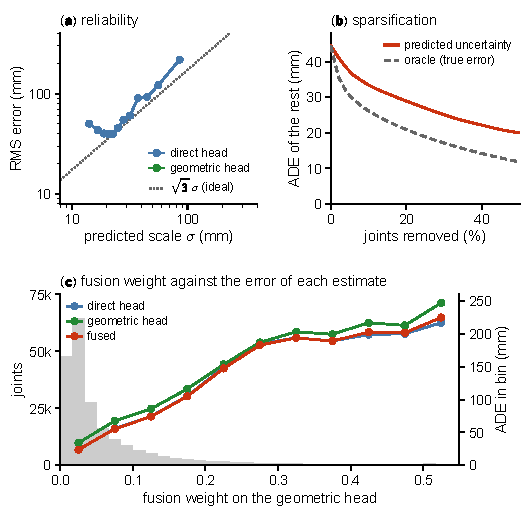
\includegraphics[width=\columnwidth]{../figures/fig7_uncertainty_FIF_hybrid_stereo_A.pdf}
\caption{The learned scales as uncertainty estimates on fold A. (a) Reliability of the direct head: predicted scale against root-mean-square error in 12 quantile bins; the geometric head's scale is constant on this fold and is shown as a single point. (b) Sparsification: discarding the 10\% of joints with the largest predicted fused scale lowers the ADE of the remainder from 44.4 to 33.4\,mm (oracle 26.2\,mm). (c) Histogram of the fusion weight on the geometric head, and the error of the direct, geometric and fused estimates as a function of that weight: the weight rises where both heads are wrong, so the fusion does not select the better head, it signals difficulty.}
\label{fig:uncertainty}
\end{figure}

\paragraph{The direct head's uncertainty is useful even where the fusion is not}
\Cref{tab:uncertainty} and \cref{fig:uncertainty} assess the learned scales as uncertainty estimates. The direct head's predicted scale correlates with its error at Spearman 0.65 on fold A and 0.63 on fold B, with a log-log reliability slope of 0.96 and 1.29, and is under-dispersed by a factor of about 1.5: its root-mean-square error is 90\,mm where an isotropic Gaussian with the mean predicted scale of 33.8\,mm would give 58\,mm, the usual over-confidence of maximum-likelihood variance heads~\cite{guo2017calibration}. Used to rank joints, it is informative: discarding the 10\% most uncertain joints reduces the ADE of the remainder from 44.4 to 33.4\,mm against an oracle of 26.2\,mm, and discarding half brings it to 20.0\,mm against 11.8\,mm; the area between the predicted and oracle sparsification curves is 7.6\,mm on fold A and 4.3\,mm on fold B. \Cref{fig:uncertainty}c shows what the fusion weight encodes: it rises where the direct head is uncertain, and there both heads are wrong by a similar amount, so the weight signals difficulty rather than picking a better estimator. A per-joint oracle that selected the better of the two heads would reach 40.75\,mm on fold A, 3.7\,mm below the achieved fusion; the geometric head is the better of the two on 28\% of joints but receives only slightly more weight there (0.075) than elsewhere (0.054), nowhere near enough to select it. Closing this gap would require the geometric head's uncertainty to be informative, which the saturation prevented.

\paragraph{The error is in the tail}
Finally, the distribution of the fused error is heavy-tailed on every fold: the median joint error is 22.6\,mm, the 90th percentile 85.9\,mm and the 99th percentile 388\,mm on fold A. The 7.9\% of joints with an error above 100\,mm carry 42.7\% of the total error, and the 3.4\% above 200\,mm carry 28.7\%. Any method that wants to move the mean substantially must address these frames, which \cref{sec:failure} shows are dominated by hands that are far from the object or outside the image.
